Trang web \emph{"https://hoadondientu.gdt.gov.vn"} do Tổng cục Thuế quản lý và sử dụng để thực hiện các quy trình liên quan đến hóa đơn điện tử. Thực tế, yêu cầu đăng ký và phê duyệt chính thức từ Tổng cục Thuế dành cho cá nhân và doanh nghiệp. Trong đồ án này, em sẽ tạo một phiên bản giả lập là \emph{"tct-demo"}, dành cho mục đích học tập phục vụ cho bài toán chính là \emph{"Xây dựng kiến trúc vi dịch vụ cho bài toán quản lý hóa đơn điện tử"}.

Trong phiên bản giả lập, em có chức năng đơn giản là \emph{"Tạo uuid"} hoặc \emph{"Không chấp nhận tạo uuid"} dùng để nhận yêu cầu định danh tài khoản và hóa đơn từ phần mềm quản lý hóa đơn điện tử.

\begin{figure}[H]

\centering

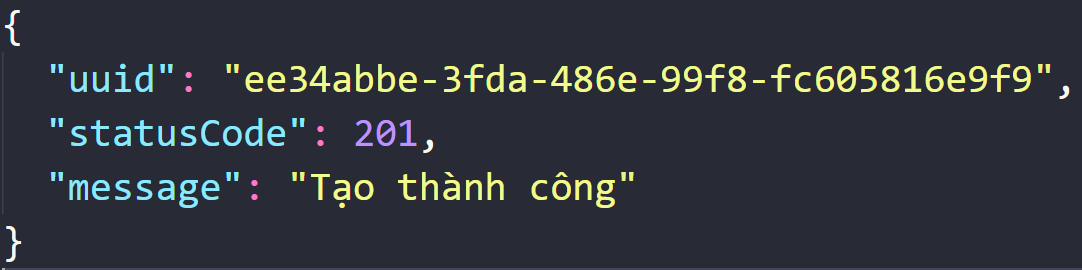
\includegraphics[scale = 0.5]{pictures/_ket_qua_tao_thanh_cong_uuid/main.png}

\caption{Kết quả tct-demo tạo thành công uuid}

\end{figure}

\begin{figure}[H]

\centering

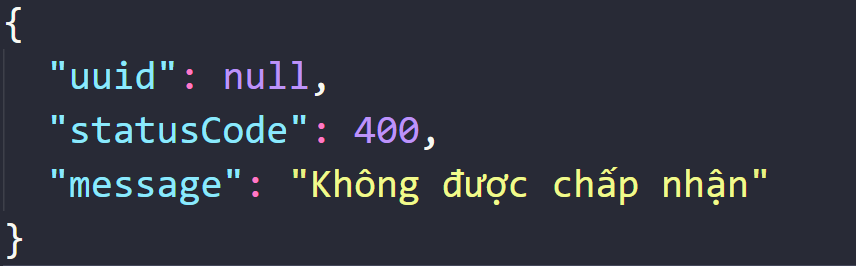
\includegraphics[scale = 0.5]{pictures/_ket_qua_tao_khong_thanh_cong_uuid/main.png}

\caption{Kết quả tct-demo tạo không thành công uuid}

\end{figure}